\documentclass{pnu-survey}


% 이미지 및 그래프 관련 패키지
\usepackage{graphicx}
\usepackage{float}
\usepackage{subfloat}
\usepackage{subfigure}
\usepackage{lscape}
\usepackage{enumitem}

% \usepackage[compact]{titlesec}

% 수학 기호 관련
\usepackage{gensymb}
\usepackage{amsmath}
\usepackage{amssymb}
\usepackage{amsthm}
\usepackage{exscale}
\usepackage{textcomp}

\newcommand{\cl}[1]{\textcircled{\scriptsize #1}}

% 알고리즘 표현
\usepackage{algorithmic}
\usepackage{algorithm}

% customize algorithmic environment
\renewcommand{\algorithmicrequire}{\makebox[40px]{\hfill\textbf{Input :}}}
\renewcommand{\algorithmicensure}{\makebox[40px]{\hfill\textbf{Output :}}}

% 테이블 관련
\usepackage{array}
\usepackage{tabulary}
\usepackage{multirow}
\usepackage[table]{xcolor}
\usepackage{ctable}
\usepackage{booktabs}
							
% 제목, 저자, 요약
\title{Puppet, Chef, Ansible의 특징 및 비교}
\author{여지수(duwltn1301@pusan.ac.kr)}
\abstract{
기업들의 인프라 환경이 복잡해지면서 인프라를 자동적으로 관리하는 기술인 “IaC(Infrastructure as Code)”에 대한 관심이 꾸준히 증가하고 있다. 이전에는 일일이 해야했던 수작업들에 대해 자동화하여, 반복적인 작업을 최소화하고 IT 인프라를 보다 빠르고 안전하며 일관되게 제공할 수 있다. 빠르고 복잡한 프로비저닝에 대한 수요의 증가로, IaC를 구현하고자 하는 여러 소프트웨어 구성 관리 툴들이 개발이 되었다. 본 논문은 인프라 구성관리도구들 중 Puppet, Chef, Ansible의 특징들을 분석하고 비교함으로써 IaC를 이해하고자 한다.}

\begin{document}

\maketitle

\section{서론}

지난 수십년 간 시대가 변화되면서 규모가 큰 기업들은 다양한 시스템 환경을 구성하고 복잡한 구조의 네트워크를 이루게 되었다. 관리자의 입장에서 다수의 시스템 환경이 동시다발적으로 문제를 일으킨다면, 그러한 각각의 시스템 환경들에서 수동으로 서버를 관리하기란 쉽지않다. 이를 해결하기 위해 “코드형 인프라”라는 개념이 등장한다. ~\cite{iac}“코드형 인프라(Infrastructure as Code, IaC)는 수동 프로세스가 아닌 코드를 통해 인프라를 관리하고 프로비저닝하는 것”을 말한다. IaC로 인프라 프로비저닝을 자동화함으로써 서버를 배포할 때마다 관리자가 직접 각각의 시스템 환경들에 대해 수동으로 프로비저닝을 할 필요가 없어진다. 관리자는 IaC의 도구를 이용해 서버 설계, 설치, 환경설정 및 관리를 자동화시킴으로써 인프라 구성을 관리할 수 있다. 이 도구를 통해 관리자가 각각의 서버에 대한 최적의 시스템 환경 설정을 정의하는 ‘코드’를 만들어 push를 하면, 다수의 시스템 환경을 편리하게 관리할 수 있게 된다. 이 논문에서는 이러한 인프라 구성관리도구 중 Puppet, Chef, Ansible의 특징들에 대해 분석하고 차이들을 비교할 것이다.

\section{본론}

\subsection{Puppet}

Puppet은 2005년 Luke Kanies가 설립한  Puppet Labs에서 개발된 형상관리를 위한 도구~\cite{puppet}로 CM 시장에서 가장 큰 점유율을 차지한다. Oracle과 Google과 같은 유명 기업들이 Puppet을 이용해 데이터 서버를 운영하고 있다. Puppet은 Ruby로 개발되었고, '서버-클라이언트' 구조를 가진다. 프로그램 설정에 필요한 데이터들은 “Module”이라는 곳에 보관이 된다. PUPPET은 서버(master)에서 이 Module을 작성하고 배포하면, 클라이언트(agent)는 설치 후 서버에 보고를 하는 식의 형태를 띤다. 

Puppet의 구조를 그림\ref{fig:puppet}으로 나타냈다. Puppet의 구성요소에는 manifest, template, file, puppet master, puppet client, agent, factor 가 있다.  
\begin{figure}[!ht]
\centering
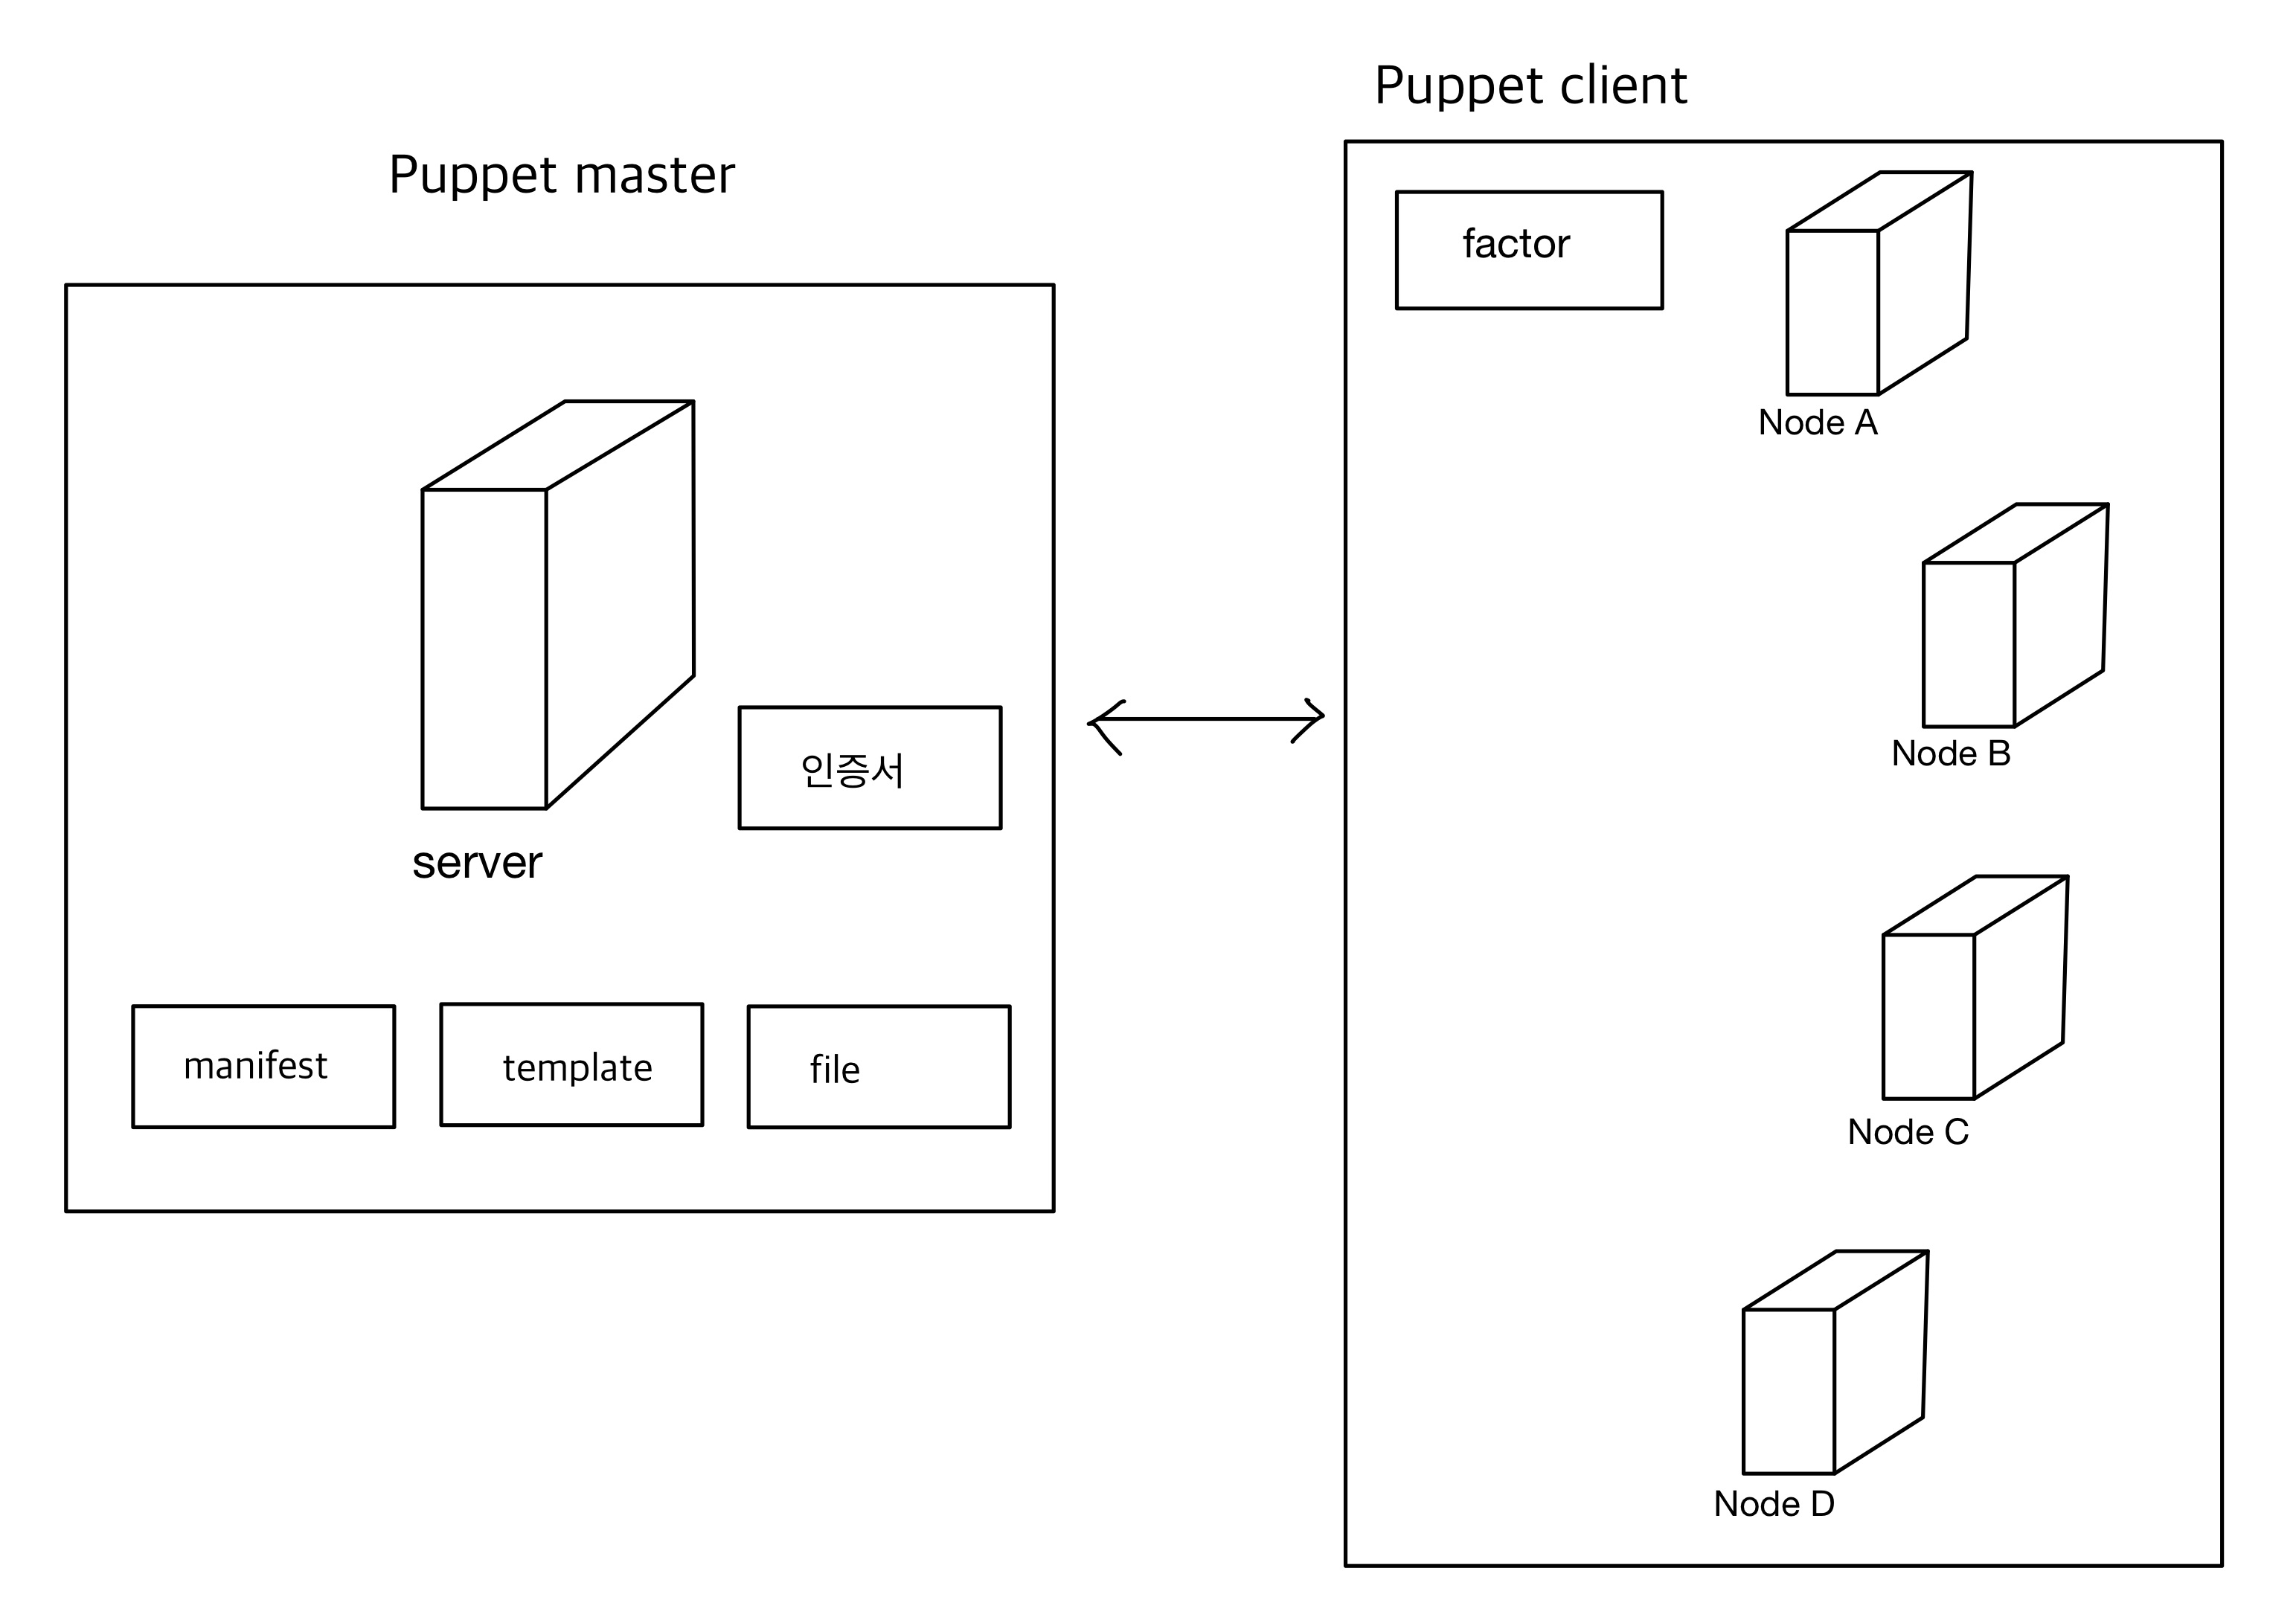
\includegraphics[width=0.4\textwidth]{img/puppet.jpg}
\caption{puppet을 이용한 architecture}
\label{fig:puppet}
\end{figure}
\index{figure}

\begin{itemize}[itemsep=0pt,parsep=0pt]
    \item manifest: 클라이언트의 구성을 설정하는 ruby로 된 코드이다.
    \item template: 코드를 수집하고 문서화한 자료이다.
    \item file: 실제 배포 되어지는 내용이다.
    \item puppet master: 모듈들(manifest, template, file)로 이루어진 시스템 주요 구성관리 파일(main configuration files)을 포함한다.
    \item puppet client: 환경 설정의 대상이 되는 디바이스이다.
    \begin{itemize}
        \item agent: 마스터 서버와 지속적으로 인증확인을 위해 교신하는데 이용된다.
        \item factor: 클라이언트의 현재 구성 설정 정보를 모아서 마스터 서버로 보내준다.
    \end{itemize}
\end{itemize}

클라이언트는 에이전트를 통해서 마스터 서버와 지속적으로 상호교신을 한다. 
에이전트는 클리이언트의 기기 ID와 인증서를 마스터 서버에 보내고, 마스터 서버는 인증서에 인증 사인을 해서 클라이언트에 회신한다. 이로써 안전하고 상호 확인되는 파일 및 정보를 교환할 수 있다.
이렇게 마스터서버와 클라이언트 간에 상호 인증이 이루어지면 클라이언트는 현재 구성 설정 정보를 알려주는 fact를 마스터 서버에 보낸다. 마스터 서버는 이 fact를 이용하여 manifest를 카탈로그로 만든 다음 각각의 클라이언트로 전송한다. 클라이언트의 에이전트는 카탈로그에 있는 manifest를 수행하여 시스템 업데이트를 하게 된다. 업데이트가 끝난 후 에이전트는 마스터 서버에 보고서를 보내 클라이언트에 설치된 소프트웨어에 대한 최신 정보를 업데이트 시켜준다.

\subsection{Chef}
Chef~\cite{chef}는 2009년 Ruby로 개발된 형상관리를 위한 프레임워크이다. 
실제로 프레지, 페이스북과 같은 유명한 기업들이 이 Chef를 사용한다. 
Puppet에서는 Module이 설정에 필요한 데이터들을 보관한다면, Chef에서는 ‘Cookbook’이 그 역할을 맡고 있다. 
Chef는 ‘서버-클라이언트’구조에 “workstation”이 추가된 구조이다. 
서버는 Cookbook을 보관하는 역할만 하며, workstation에서 Cookbook을 개발하고 서버에 업로드하며 배포 지시를 내린다.  
클라이언트(node)는 서버로부터 데이터를 가져와 패키지를 설치하고 애플리케이션을 실행한다.

Chef의 구조를 그림\ref{fig:chef}로 나타냈다. 
\begin{figure}[!ht]
\centering
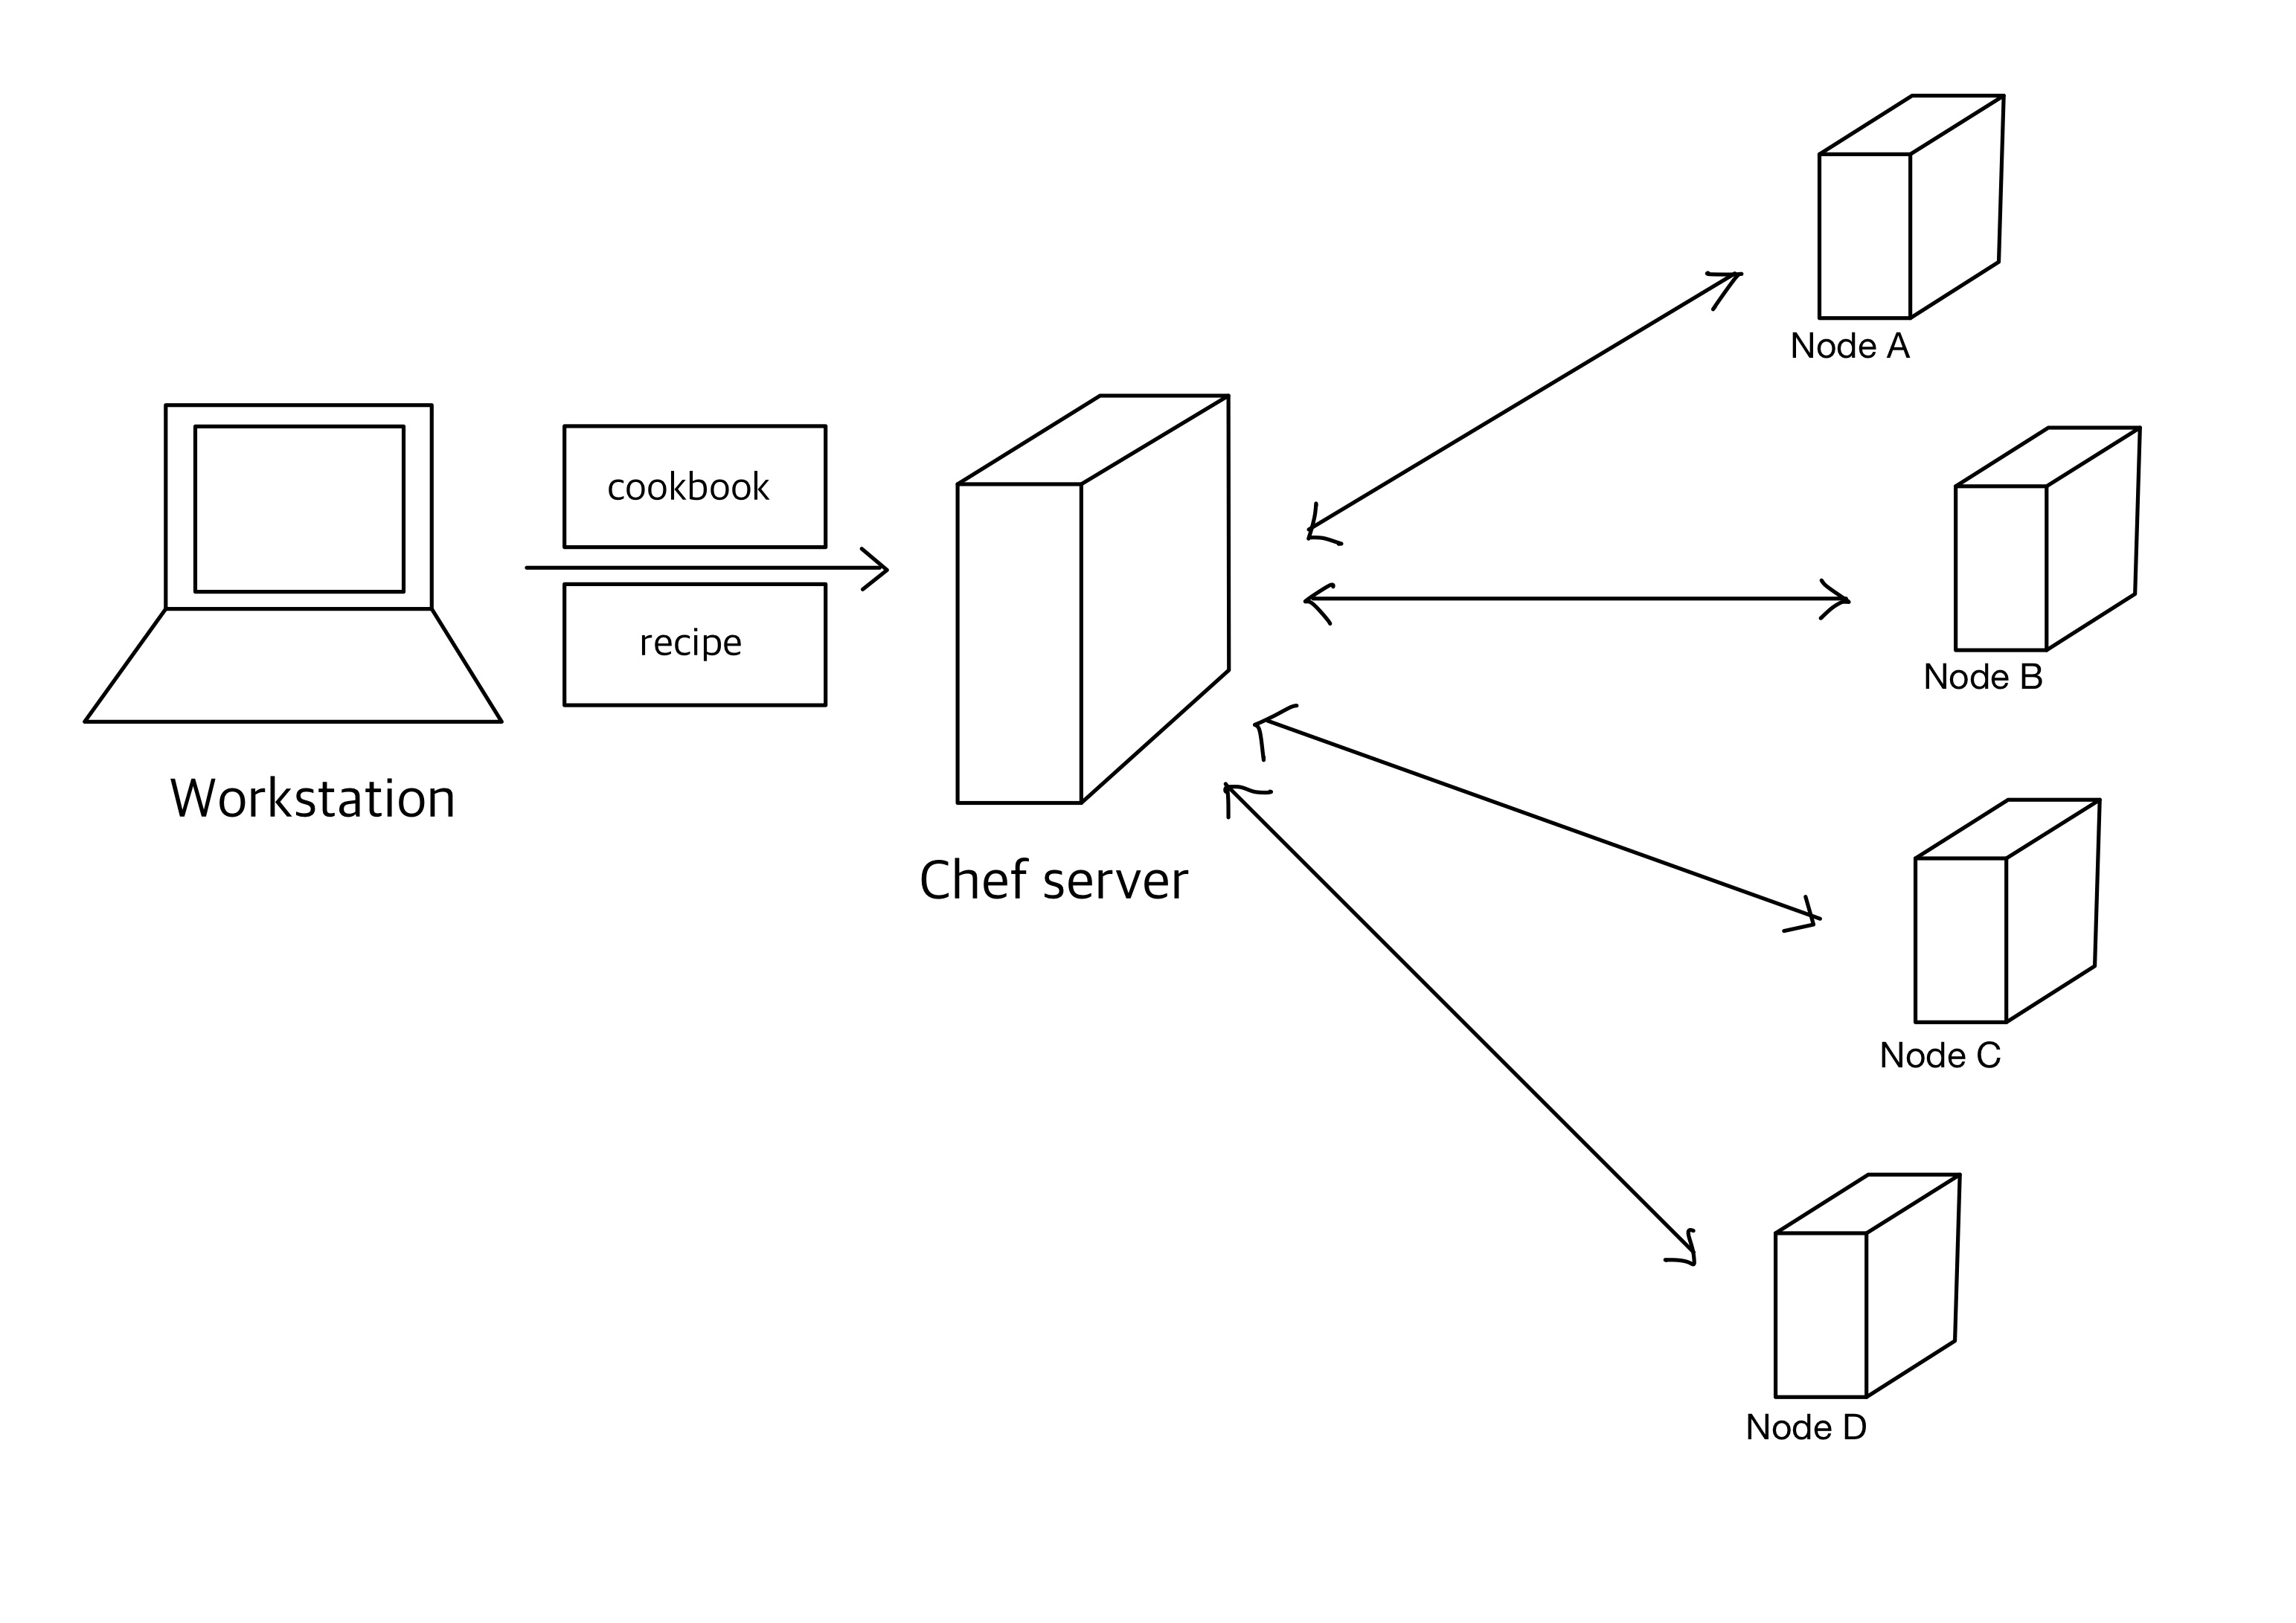
\includegraphics[width=0.4\textwidth]{img/chef.jpg}
\caption{chef을 이용한 architecture}
\label{fig:chef}
\end{figure}
\index{figure}

Chef의 구성요소에는 workstation, recipe, cookbook, knife, server, node가 있다.  
\begin{itemize}[itemsep=0pt,parsep=0pt]
    \item recipe: 시스템 구성설정 및 업데이트를 위해 ruby로 작성된 스크립트이다.
    \item cookbook: 다수의 레시피를 모아둔 것이다.
    \item knife: recipe와 시스템 간 communication을 할때 사용하는 명령문 (command)이다.
    \item node: 회사 네트워크에 연결된 컴퓨터 장비이다.
\end{itemize}
관리자는 knife를 이용해 Chef 서버에 달린 여러 노드들의 현재 시스템 환경 설정 상태를 상시적으로 확인한다. 그리고 필요에 따라 recipe를 작성해서 서버에 보내게 된다. 관리자는 자신의 로컬 workstation에서 각각의 노드에서 설정되어야 할 구성들에 관해 recipe를 작성한다. recipe는 cookbook에 저장되어 Chef 서버에 전달되고, 해당 서버는 각각의 노드에게 맞는 recipe를 배치함으로써 노드의 환경을 새롭게 설정하게 된다. 

\subsection{Ansible}
Ansible~\cite{ansible}은 2012년 Python으로 개발된 것으로 현재 Red Hat이 소유하고 있다. Puppet에 비해 훨씬 작은 시장 점유율을 가진다.
기존의 구성 관리 도구인 Chef와 Puppet은 중앙의 서버에 접근해 설정에 관한 정보를 가져왔다. 이 방식을 pull type 아키텍쳐라고도 하는데, Ansible 같은 모델은 push type 아키텍쳐이다. 중앙의 머신이 SSH를 이용한 네트워크 접속 방식으로 각각의 노드에 로그인을 해서 직접 명령을 실행하는 방식이다. 

Ansible의 구조를 그림\ref{fig:ansible}로 나타냈다. 
\begin{figure}[!ht]
\centering
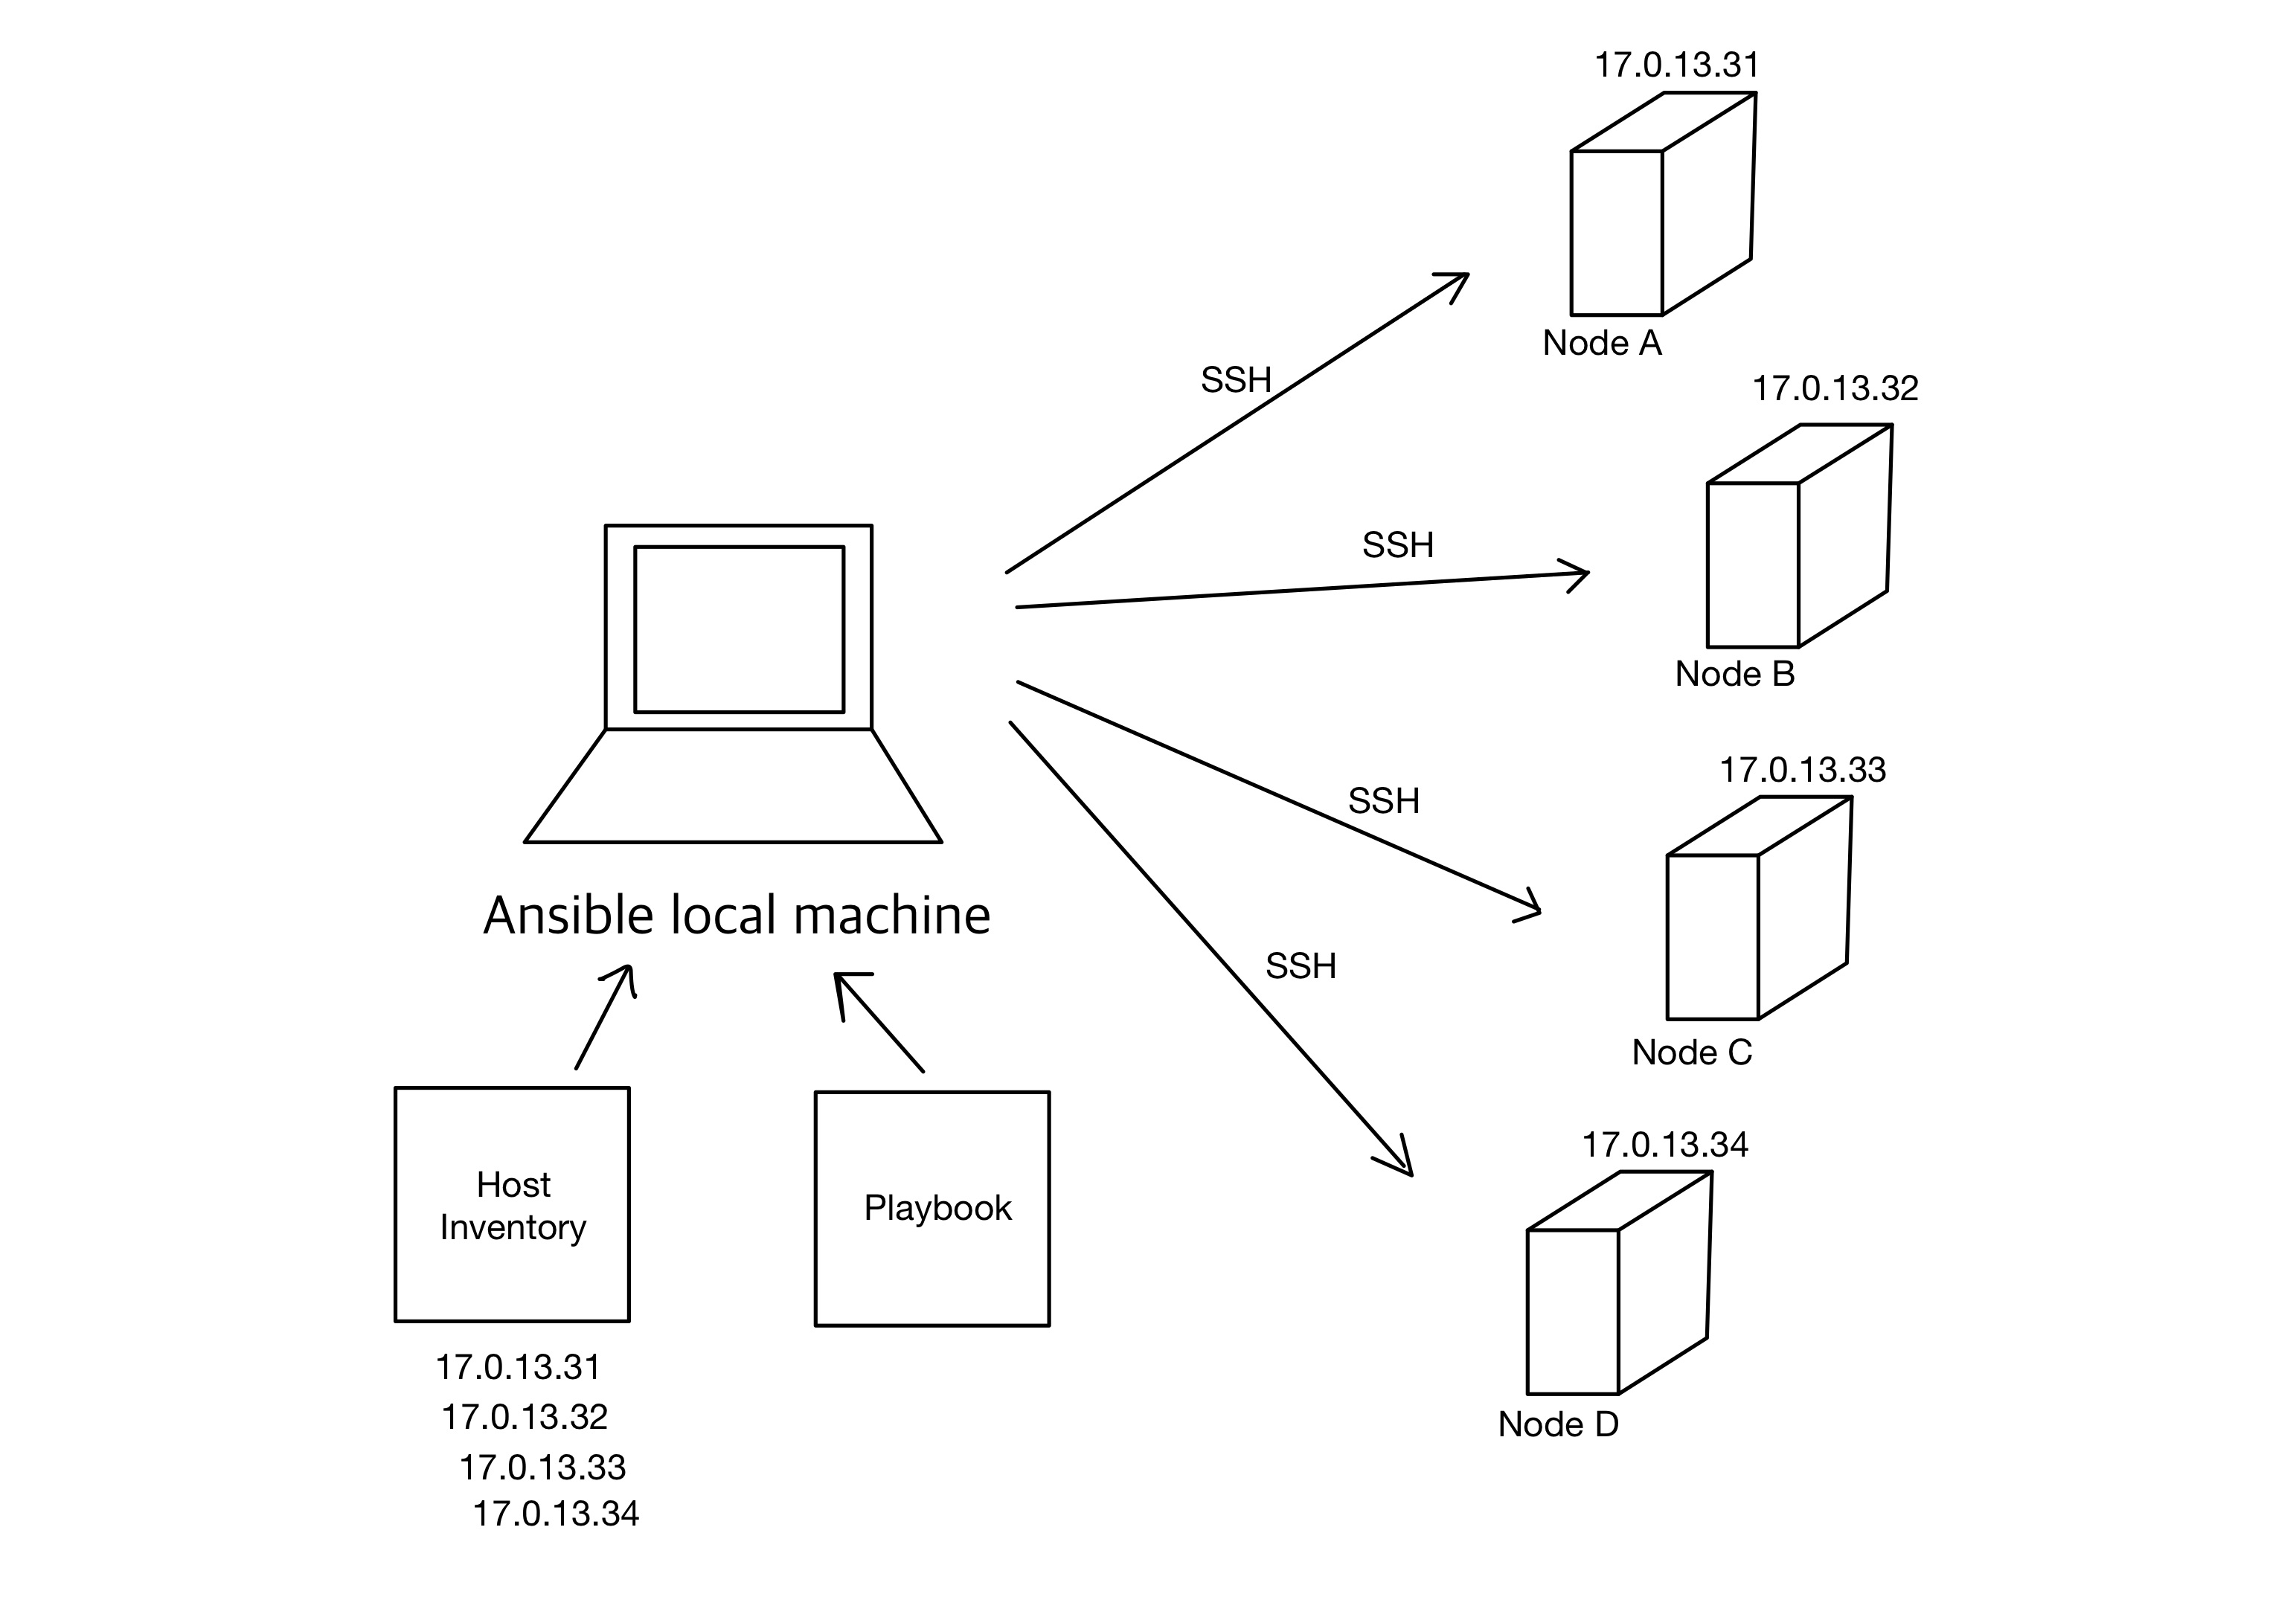
\includegraphics[width=0.4\textwidth]{img/ansible.jpg}
\caption{ansible을 이용한 architecture}
\label{fig:ansible}
\end{figure}
\index{figure}

Ansible의 구성요소에는 inventory, module, playbook, local machine, node 가 있다.  
인벤터리는 여러 개의 서버를 그룹화해 정의하거나 각각의 서버와 그룹에 대해 변수를 사용한 파라미터를 설정할 수 있다.

\begin{itemize}[itemsep=0pt,parsep=0pt]
    \item Inventory: 설정 대상이 되는 서버의 접속 정보를 나타낸다.
    \item Module: 개별적인 작업들에 대해 명령어로 정의한다. 
    \item Playbook: 시스템 구성설정 및 업데이트를 위해 python 또는 yaml으로 작성된 스크립트이다.
\end{itemize}

하나의 로컬 머신은 인벤토리 파일과 플레이북에 대한 정보를 가지고 있다.
인벤토리 파일에는 서버가 연결해야 하는 노드를 알 수 있도록 노드의 IP가 저장되어 있다.
플레이북이 작성되면 SSH를 통해 노드들로 푸시되고 마스터 노드는 각 노드에 대한 정보를 수집하고 분석한다.
플레이북에 작성된 작업이 실행되고 필요한 구성이 관리된다.

\subsection{차이점}

puppet과 chef는 DSL 방식인 ruby를 사용하고, ansible은 CLI 방식인 파이썬을 사용한다~\cite{difference}. puppet과 chef는 마스터-클라이언트 구조이고, 여기서 chef는 workstation이 추가된 구조이다. ansible은 마스터로 이루어진 구조이다. puppet과 chef는 pull 방식의 모델이고, ansible은 push 방식의 모델이다. puppet과 chef는 인증 방식으로 SSL을 취하고, ansible은 SSH를 통해 노드에 접근한다. 난이도는 보다 최근에 나온 ansible이 puppet과 chef에 비해 가볍고 배포가 빨라 쉽고, 확장성도 매우 높은 편이다. 그러나 ansible은 chef와 puppet에 비해 훨씬 작은 시장 점유율을 가진다. Puppet은 오류가 있는 경우 작업을 실행하기 전에 쉽게 강조를 표시할 수 있으나, Ansible에서는 작업이 순서대로 실행되기에 해당 작업이 실행이 될 때까지 작업이 실패를 할 지에 대한 여부를 알 수가 없다. 

표 \ref{tab:difference}를 통해 Puppet, Chef, Ansible의 차이점에 대해 작성해보았다. 
\begin{table}[!ht]
\centering
\setlength{\belowcaptionskip}{5pt}
\caption{Chef, Puppet, Ansible 차이}
\label{tab:difference}
\begin{tabular}{@{}lrrrr@{}} 
\toprule
{\bfseries Category} & {Puppet} & {Chef} & {Ansible} \\
\midrule
언어			    &Ruby	            &Ruby		            &Python\\
구조		        &Master-Agent	    &Master-Agent 		    &Master \\
관리 방식		    &Pull	            &Pull		            &Push \\
통신 			&SSL                &SSL                    &SSH \\
난이도			&어렵다		        &어렵다		            &쉽다 \\
확장성			&높다			    &높다		            &매우 높다 \\
시작연도			&2005			    &2009		            &2012 \\
\bottomrule
\end{tabular}
\end{table}


\section{결론}
지금까지 Puppet, Chef 와 Ansible을 여러 카테고리별로 간단하게 비교를 해보았다. puppet과 chef는 workstation이라는 차이를 제외하면 비슷한 부분이 많았고, ansible은 앞의 두 도구와 많은 차이를 보였다. ansible은 puppet과 chef와 달리 Agent가 없는 방식으로 보다 단순하여 설정이 쉽고 빠른편이다. 하지만 아직 시장 점유율이 작으며, 작업에 오류가 있는 경우 작업이 실행이 될 때까지 작업이 실패할 지에 대한 여부를 알 수 없다.

이로써 관리자가 서버들의 환경 설정을 반복적으로 해야할 때 이와 같은 구성관리도구들을 통해 IaC~\cite{iac}를 구현하면 빠르고 안정적이게 설정을 마칠 수 있다. 그리고 소수의 시스템 관리자만 통제할 수 있는 것이 아닌, 개발자 스스로가 인프라를 통제할 수 있는 환경으로 만들 수 있기에 이를 활용한 플랫폼들이 증가될 것으로 보인다. 

\bibliographystyle{ieeetr}
\bibliography{ref}
\end{document}


